\subsection{Tipo de entidad Asignatura Curso Académico}

   \begin{description}

   \item[Definición] Se refiere al objeto del mundo real: \emph{``Asignatura
   impartida en un determinado curso académico''}.

   \item[Características] La entidad presenta las siguientes características:
      \begin{itemize}
         \item \textbf{Nombre:} Asignatura Curso Académico.
         \item \textbf{Tipo:} Débil por identificación con respecto a Asignatura.
         \item \textbf{Número de atributos:} 1 propio y 3 heredados.
         \item \textbf{Atributo/s identificador/es principal/es:} id\_centro junto con \\id\_titulación, id\_asignatura y curso\_académico.
         \item \textbf{Atributo/s identificador/es alternativo/s:} -
         \item \textbf{Atributo/s heredado/s:} id\_centro, id\_titulación e
         id\_asignatura del tipo de entidad Asignatura.
      \end{itemize}

   \item[Diagrama] La figura \ref{diagramaACA} muestra el diagrama de la entidad.
   \item \begin{figure}[!ht]
            \begin{center}
            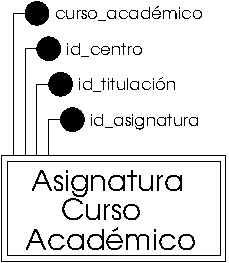
\includegraphics[]{07.Modelo_Entidad-Interrelacion/7.2.Analisis_Entidades/diagramas/aca.pdf}
            \caption{Diagrama de la entidad Asignatura Curso Académico.}
            \label{diagramaACA}
            \end{center}
         \end{figure}

   \item[Descripción de los atributos propios] Esta entidad presenta el
   siguiente atributo propio:

   \begin{itemize}
   \item \textbf{curso\_académico}
      \begin{itemize}
         \item \textbf{Definición:} Hace referencia al periodo de tiempo en que se imparte una determinada asignatura.
         \item \textbf{Dominio:} Formato de fecha: aaaa. Estos cuatro dígitos determinan el año de inicio del curso académico al que se hace referencia.
         \item \textbf{Carácter:}  Obligatorio.
         \item \textbf{Ejemplo práctico:} 2008.
         \item \textbf{Información adicional:} El dato lo proporciona el usuario alumno al establecer las asignaturas en las cuales se ha matriculado. Es la clave primaria junto con id\_centro, id\_titulación e id\_asignatura.
      \end{itemize}
   \end{itemize}

   \item[Ejemplo práctico]

   \item \begin{center}
            \begin{tabular}{ | l | l | }
            \hline
            \multicolumn{2}{ | c | }{\textbf{Tipo de entidad Asignatura Curso Académico}} \\
            \hline
            id\_centro & 15 \\
            \hline
            id\_titulación & 3\\
            \hline
            id\_asignatura & 17\\
            \hline
            curso\_académico & 2008\\
            \hline
            \end{tabular}
         \end{center}
   \end{description}
